\chapter{Konzeption der Megamap-Anwendung}
\label{chap:concept}
Dieses Kapitel beschreibt die Konzeption der im Rahmen dieser Arbeit entwickelten Megamap-Anwendung.
Da in dieser Arbeit die Kartenexploration im Gegensatz zur -navigation stärker fokussiert wird, wird zunächst der Begriff der Kartenexploration definiert.
Um zu verstehen, wie eine digital unterstütze Kartenexploration umgesetzt werden kann, werden Elemente zur Kartenexploration aus bereits existierenden Kartenanwendungen herausgearbeitet.
Diese Elemente werden kategorisiert, zusammengefasst und schließlich als Grundlage für das Megamap-Konzept verwendet.
%Schließlich wird ein Überblick der für die Implementierung benötigten Komponenten gegeben.

\section{Definition Kartenexploration}
\label{sec:definition_exploration}
% Hier die Guidelines einarbeiten
Bereits \textcite{Reichenbacher2001} beschreibt Konzepte zur mobilen Nutzung von digitalen Kartensystemen.
Er gibt eine Übersicht verschiedener \emph{User Tasks}, die in mobilen Umgebungen ausgeführt werden können (siehe \autoref{tab:gis_user_tasks}).
Einer dieser User Tasks ist die \textbf{Navigation}, welcher in digitalen Kartensystemen durch Wegbeschreibungen umgesetzt wird.
Nutzer bekommen einen oder mehrere Pfade zwischen zwei Punkten angezeigt, welche den Nutzern z.B. den schnellsten oder den kürzesten Weg zum Ziel anschaulich machen.
Zusätzlich können wegweisende Textinformationen die Navigation erleichtern.

Neben der Navigation nennt \citeauthor{Reichenbacher2001} drei weitere Kategorien von User Tasks:

\textbf{Lokalisierungs-Tasks (\emph{Locators})} sind Anwendungsfälle, bei denen Nutzer Positionen abfragen und diese angezeigt werden.
Dabei kann es sich um die eigene Position handeln, aber auch um die von anderen Personen oder Objekten.

\textbf{Nähe-Tasks (\emph{Proximity})} sind Anwendungsfälle, bei denen Nutzer Informationen über die Umgebung relativ zur eigenen Position erhalten.
So können Nutzer z.B. die Umgebung nach den nächstgelegenen Geschäften oder Freizeitbeschäftigungen abfragen.

\textbf{Events} sind nicht nur ortsabhängig, sondern auch zeitabhängig.
Bei diesen Anwendungsfällen geht es um die Abfrage von Informationen, die sich mit der Zeit ändern.
Z.B. fallen die Abfrage von geöffneten Geschäften oder von Verkehrsinformationen in diese Kategorie.

Eine Gemeinsamkeit dieser Anwendungsfälle ist, dass hier Informationen über die Umgebung abgefragt werden.
Die Informationen sind abhängig von \emph{mindestens} einem Kontext, zum Beispiel der aktuellen Position der Nutzers.
Es können aber auch mehrere Kontexte gleichzeitig mit einbezogen werden (Beispiel: \enquote{Alle \emph{Geschäfte} in \emph{der Nähe}, die \emph{zurzeit} geöffnet sind} $\rightarrow$ Zweck-, Positions- und Zeitkontext).
Dies steht im Kontrast zur Navigation, für welche immer ein Endpunkt im Kontext zu \emph{mindestens} einem Startpunkt stehen muss (weitere Kontexte wären z.B. Zwischenstopps, das genutzte Fortbewegungsmittel oder das aktuelle Verkehrsaufkommen).

Da Nutzer eine Umgebung durch Abfragen ihrer Informationen \enquote{entdecken}, wird in dieser Arbeit \textbf{Kartenexploration} als Oberbegriff für die Lokalisierungs-, Nähe- und Event-Tasks betrachtet.
Somit grenzt sich die Kartenexploration von der reinen Navigation durch die zuvor beschriebenen Unterschiede ab.

\begin{table}[tbh]
    \centering
    \caption{Geoinformationsaufgaben in einer mobilen Umgebung. \quelle{\cite[47]{Reichenbacher2001}}}
    \label{tab:gis_user_tasks}
    \begin{tabular}{@{}lll@{}}\toprule
        \textsf{\textbf{Tasks}} & \textsf{\textbf{Subtasks}} & \textsf{\textbf{Examples}}\\ \midrule
        \multirow{3}{*}{Locators} & Own position & xy coordinates, place name \\
                                  & Objects & Attributes of an object\\
                                  & Other persons position & Who is this?\\ \midrule
        \multirow{2}{*}{Proximity} & Objects & Next object with certain attributes\\
                                   & Persons & Known people in the area?\\ \midrule
        Navigation & Routing & Way descriptions\\ \midrule
        Events & What happens at a place & Obstacles (e.g. traffic jam)?\\ \bottomrule
    \end{tabular}
    \vspace{0.5em}
\end{table}

\section{Explorationselemente in existierenden Kartenanwendungen}
Digitale Kartenanwendungen setzen unterschiedliche Elemente ein, um die Kartenexploration zu unterstützen.
Bevor das Konzept für die Megamap formuliert wird, werden die Darstellungselemente und Interaktionsmöglichkeiten zur Kartenexploration in bereits existierenden Anwendungen gesammelt und kategorisiert.
Die Idee ist, diejenigen Elemente in der Megamap zu übernehmen, welche Nutzern bereits aus den anderen Anwendungen bekannt sind.
Durch die Verwendung der bekannten Elemente und Interaktionen soll ein zusätzlicher Lernaufwand für die neuartige Megamap-Anwendung verhindert werden.
Die gesammelten Elemente und Interaktionsmöglichkeiten werden jeweils den User Tasks aus \autoref{sec:definition_exploration} zugeordnet.
Demnach ergeben sich drei Kategorien von Explorationselementen: \textbf{Lokalisierungselemente}, \textbf{Nähe-Elemente} und \textbf{Eventelemente}.

Als Beispiele für existierende Kartenanwendungen wurden die \emph{Web}-Varianten von \emph{Google Maps}, \emph{Bing Maps} \parencite{Microsoft2018b} und \emph{HERE WeGo} \parencite{HERE2018} untersucht.
Alle drei Webseiten bieten neben der Routen-Planung auch Funktionen zur Erkundung von Umgebungen an.
\autoref{tab:exploration_elements_summary} zeigt eine Übersicht der gefundenen Explorationselemente.
Die einzelnen Elemente werden in den folgenden Abschnitten mit Beispielen näher erläutert.

\begin{table}[tbh]
    \small
    \centering
    \caption{Übersicht der Explorationselemente in ausgewählten Anwendungen}
    \label{tab:exploration_elements_summary}
    \todo[inline]{TCTD aus Tabelle rausnehmen?}
    \begin{tabular}{@{}lcccc@{}}\toprule
        \textsf{\textbf{Explorationselement}} & \textsf{\textbf{Google Maps}} & \textsf{\textbf{Bing Maps}} & \textsf{\textbf{Here WeGo}} & \textsf{\textbf{TCTD}}\\ \midrule

        \multicolumn{5}{@{}l@{}}{\textsc{Lokalisierung}} \\ \midrule
        Positionsmarker (Nutzer) & \checkmark & \checkmark & \checkmark & \\
        Labels (Straßen, Flüsse, \dots) & \checkmark & \checkmark & \checkmark & \\
        Gebäudemarkierungen & \checkmark & \checkmark & \checkmark & \\
        Klickmarkierung (Adresse, Koordinaten) & \checkmark & \checkmark & \checkmark & \\
        Spezifische Suche (mittels Suchfeld) & \checkmark & \checkmark & \checkmark & \\

        \midrule
        \multicolumn{5}{@{}l@{}}{\textsc{Nähe}} \\ \midrule
        Gebäudemarkierungen (Positionsabh.) & \checkmark & \checkmark & \checkmark & \\
        Gebäudemarkierungen (Zoomabh.) & \checkmark & \checkmark & \checkmark & \\
        Entfernungen (außerhalb Navigation) & \checkmark & \checkmark & --- & \\
        Terrain & \checkmark & --- & --- & \\
        Nahbereichssuche & \checkmark & \checkmark & --- & \\
        Filter u. Sortierung & \checkmark & \checkmark & --- & \\
        Offene Suche (mittels Suchfeld) & \checkmark & \checkmark & \checkmark & \\
        Gebäudenachbarschaft & \checkmark & \checkmark & Nur Transport & \\
        Ausstattung (z.B. Hotels etc.)  & \checkmark & \checkmark & --- & \\
        Umgebungsbilder & \checkmark & \checkmark & --- & \\

        \midrule
        \multicolumn{5}{@{}l@{}}{\textsc{Event}} \\ \midrule
        Öffnungszeiten & \checkmark & \checkmark & \checkmark & \\
        Verkehrsinformationen & \checkmark & \checkmark & \checkmark & \\
        Veranstaltungen & \checkmark & --- & --- & \\
        Besucheraufkommen & \checkmark & --- & --- & \\

        \bottomrule
    \end{tabular}
\end{table}

\subsection{Lokalisierungselemente}
Lokalisierungselemente sind solche, die wichtige oder interessante Orte auf der Karte markieren.
Die Untersuchung der Beispielanwendungen ergab fünf Arten von Lokalisierungselementen:

Der \emph{Positionsmarker} ist ein grafisches Element auf der Karte, der die aktuelle Position des Nutzer (und unter Umständen auch die Blickrichtung) repräsentiert.
Ein Beispiel findet sich in \autoref{fig:gm_positionsmarker}.
Die Standortdienste des jeweiligen Endgeräts werden benutzt, um den Marker auf der Karte zu platzieren.
Der Positionsmarker erlaubt es dem Nutzer, seine eigene Position in der Umgebung zu bestimmen.

\emph{Labels} sind Textelemente, welche die Namen von Straßen, Flüssen, Gebäuden etc. auf der Karte zeigen (siehe \autoref{fig:hwg_labels}).
Nutzer können Kartenlabels mit Schildern und Wegweisern in der Umgebung abgleichen, was die Orientierung erleichtert.
Zudem sind Wegbeschreibungen deutlicher, wenn Orte auf der Karte und in der Umgebung explizit benannt werden können.

\emph{Gebäudemarkierungen} sind grafische Elemente, welche die Positionen von gewissen Gebäuden auf Karten markieren.
Es gibt sowohl statische Gebäudemarkierungen, die zusammen mit den Labels auf der Karte fest verankert sind, wie auch dynamische Gebäudemarkierungen, die je nach Kontext des Nutzers ein- bzw. ausgeblendet werden.
Die dynamischen Gebäudemarkierungen werden durch sogenannte \enquote{Stecknadeln} repräsentiert.
Diese sind mit Icons versehen, welche die Kategorie des Gebäudes anzeigen.
Beispiele finden sich in \autoref{fig:bm_gebaeudemarkierungen}.

Eine \emph{Klickmarkierung} kann in den Kartenanwendungen durch Klicken auf den Kartenbereich erzeugt werden.
Die Markierung wird grafisch als Stecknadel oder ein vergleichbares Symbol dargestellt (siehe \autoref{fig:gm_klickmarkierung}).
Über eine solche Markierung kann der Nutzer auf die Adresse und / oder die Koordinaten am angeklickten Ort zugreifen.

Die \emph{spezifische Suche} ist eine Lokalisierungs-Interaktion, die durch ein Suchfeld ausgelöst wird.
Als \emph{spezifische} Suche (im Gegensatz zur \emph{offenen} Suche) wird in dieser Arbeit die Suche nach einer bekannten Adresse oder einem eindeutig benannten Ort verstanden (beispielsweise \enquote{Bremer Rathaus} oder \enquote{Bibliothekstraße 1}).
Wird eine solche Suche durchgeführt, platziert die Anwendung eine grafische Markierung auf dem Zielobjekt.
Den Nutzern bleibt somit eine manuelle Suche nach dem Zielort auf der Karte erspart.

\begin{figure}
    \centering
    \begin{minipage}[t]{.485\textwidth}
        \centering
        \vspace{0pt}
        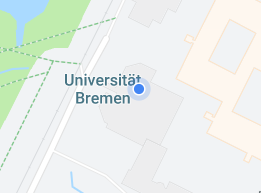
\includegraphics[width=\linewidth, height=4.5cm]{figures/map-app_examples/gm_positionsmarker}
        \captionof{figure}{Beispiel eines Positionsmarkers in Google Maps.}
        \label{fig:gm_positionsmarker}
        \vfill
    \end{minipage}
    \hfill
    \begin{minipage}[t]{.485\textwidth}
        \centering
        \vspace{0pt}
        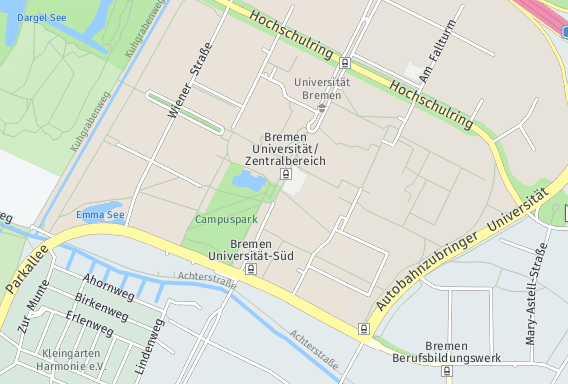
\includegraphics[width=\linewidth, height=4.5cm]{figures/map-app_examples/hwg_labels}
        \captionof{figure}{Beispiel von Labels in HERE WeGo.}
        \label{fig:hwg_labels}
    \end{minipage}
\end{figure}

\begin{figure}
    \centering
    \begin{minipage}[t]{.485\textwidth}
        \centering
        \vspace{0pt}
        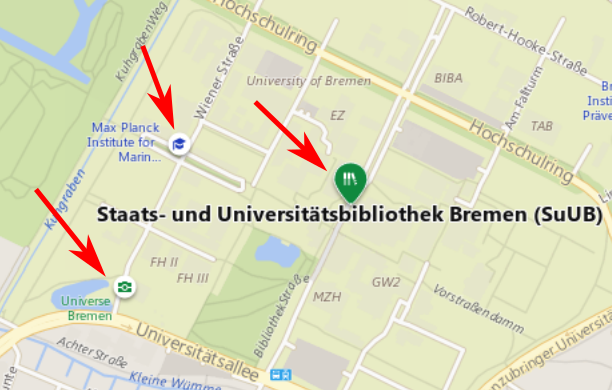
\includegraphics[width=\linewidth, height=4.5cm]{figures/map-app_examples/bm_gebaeudemarkierungen_arrows}
        \captionof{figure}{Beispiel von Gebäudemarkierungen in Bing Maps (hervorgehoben durch \textcolor{red}{rote} Pfeile). %
        Ausgewählte Orte werden durch Stecknadeln stärker betont.}
        \label{fig:bm_gebaeudemarkierungen}
        \vfill
    \end{minipage}
    \hfill
    \begin{minipage}[t]{.485\textwidth}
        \centering
        \vspace{0pt}
        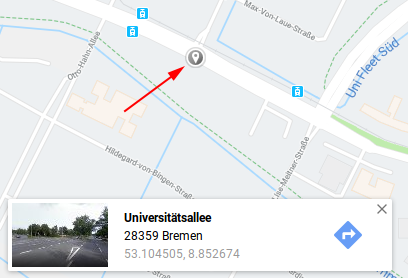
\includegraphics[width=\linewidth, height=4.5cm]{figures/map-app_examples/gm_klickmarkierung}
        \captionof{figure}{Beispiel der Klickmarkierung in Google Maps (hervorgehoben durch \textcolor{red}{roten} Pfeil). %
        Unterhalb der Markierung werden die Adresse und Koordinaten gezeigt.}
        \label{fig:gm_klickmarkierung}
    \end{minipage}
\end{figure}

\subsection{Nähe-Elemente}

\subsection{Event-Elemente}



\section{Megamap in \emph{Tom Clancy's The Division}}
% Mechanics

\section{Anwendung der Explorationselemente für Megamap}

%
\cleardoublepage
